\documentclass{article}
\usepackage{geometry}
\geometry{a4paper, margin=1in}
\usepackage{enumitem}
\usepackage{graphicx}
\usepackage[hidelinks]{hyperref}
\usepackage{amsmath}
\usepackage{float}
% Add any packages as you need



\begin{document}

% Cover Page
\begin{titlepage}
	\centering
	\vspace*{1cm}

	
\includegraphics[width=0.5\textwidth]{assets/logo.png}\par\vspace{1cm} % Adjust the width as needed

	\Huge
	\textbf{Proposal Title}

	\vspace{0.5cm}
	\LARGE
	Master in Statistics Mathematics

	\vspace{1.5cm}


	\textbf{Alejandro M. Ouslan}

	\vfill

	\Large
	Supervisors: \\
	Dr. Raul E. Macchiavelli \\
	Dra. Damaris Santana \\
	Dr. Julio C. Hernandez \\
	Dr. Roberto Rivera Santiago

	\vspace{0.8cm}

	\Large
	University of Puerto Rico, Mayaguez \\
	{\small \today}

\end{titlepage}


\newpage


\begin{abstract}
	This research looks to compare the preformance of Spatial regressions using a predefined
	weights matrix and semi parametric regessions with a spatila smoother
\end{abstract}
\section{Proposal Keywords}
% List your keywords separated by a comma
Spatial simulation, Spatial Regressions, GAMs, Tensor Products

\section{Introduction}

Regressions are use to simplfy and model complex relationship of the real world. Every model is wrong and we add
additional compones with the objective of better representing the real world relationship. The Spatial models
shown in this paper are no different and are not a nobel consept. Through the use of simulations we are trying
to understand the limitations of this model and understand what are their limitations and show on what context
one should pick thouse models. Later next we would use some Bayesian inferecne to address one of the underlining
problems using one of the models. Finaly we will implement the model using data from the QCEW as an applied example of the
methods.


\section{Background and Motivation}

The spatial regersion are a very simple model with very express. The SDM can be express in the following model:


\section{Systematic Literature Review}

\section{Aims and Objectives}

The overall objectives of this research are to understand and compare the SDM model and Semi parametric
model using tensor products. We intend to look at on which surcumstances does each model preform better than the
other and generate better predictors closer to the truth. Additionaly we look to the cost benefits of each model
like the dificulty of immplementing teh model, asumptions, computational cost and other other observations.
\begin{equation}
	y = X \beta + \rho W X + \epsilon
\end{equation}

Where we have our classic liner componet of $X\beta$ plus our spatial componet $\rho W X$. This is the data generating
process,the $W$ is a matrix that the researcher knows and chooses. However in practice the researcher does not know how
this process is conducted and needs to infer what type of realationships does $W$ represent. For example this $W$ can be represened
in the following ways:

\begin{figure}[H]
	\centering
	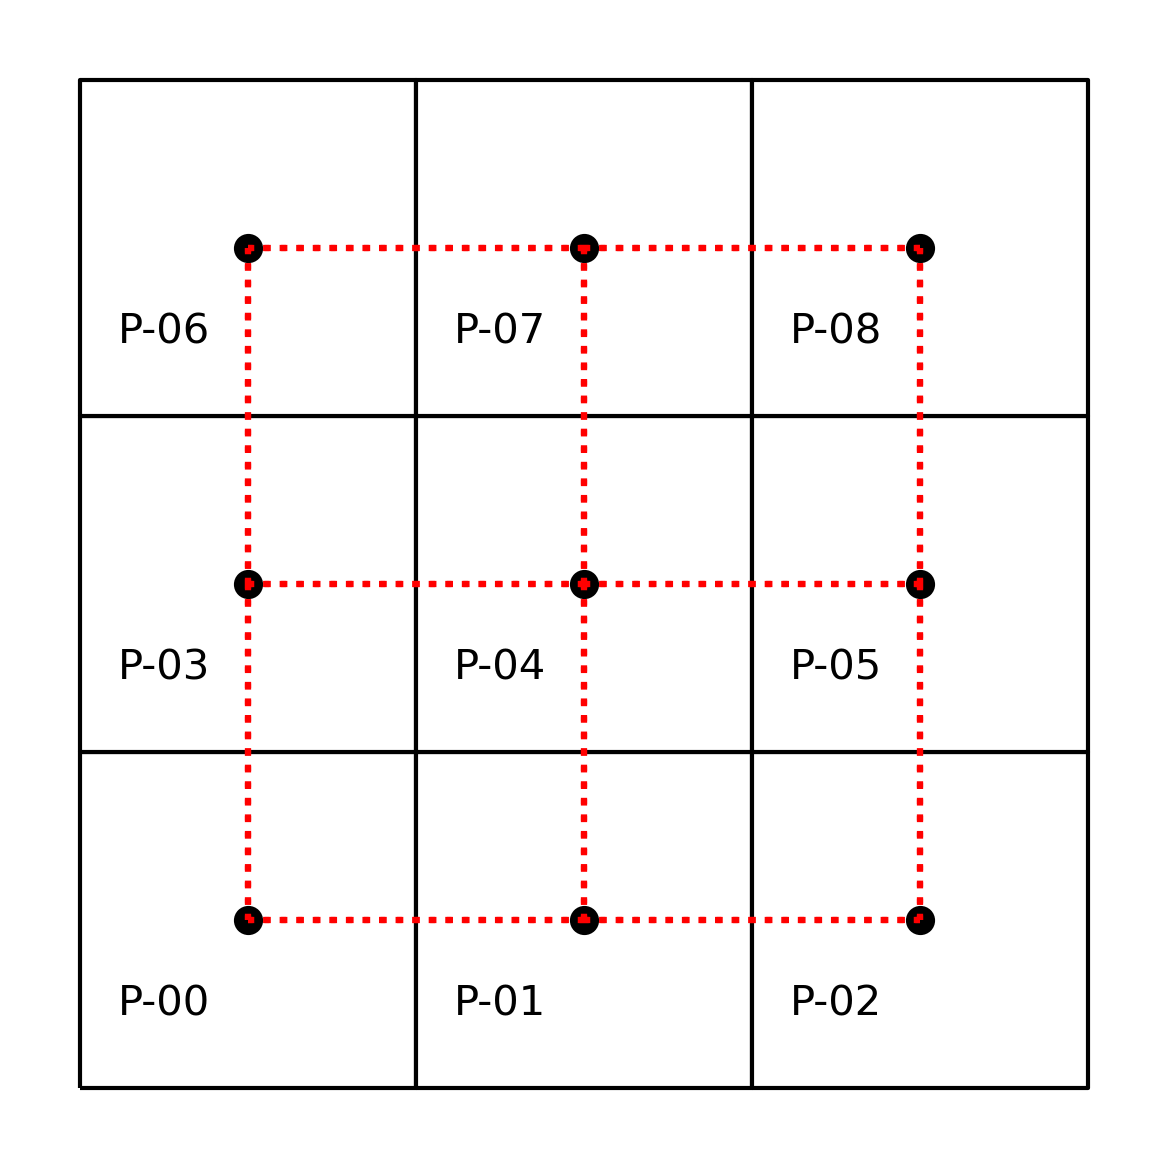
\includegraphics[width=0.4\textwidth]{assets/rook.png}
	\caption{Rook Model}
\end{figure}


Represented mathematicaly this would be the following matrix

\[
	\begin{bmatrix}
		0 & 1 & 0 & 1 & 0 & 0 & 0 & 0 & 0 \\
		1 & 0 & 1 & 0 & 1 & 0 & 0 & 0 & 0 \\
		0 & 1 & 0 & 0 & 0 & 1 & 0 & 0 & 0 \\
		1 & 0 & 0 & 0 & 1 & 0 & 1 & 0 & 0 \\
		0 & 1 & 0 & 1 & 0 & 1 & 0 & 1 & 0 \\
		0 & 0 & 1 & 0 & 1 & 0 & 0 & 0 & 1 \\
		0 & 0 & 0 & 1 & 0 & 0 & 0 & 1 & 0 \\
		0 & 0 & 0 & 0 & 1 & 0 & 1 & 0 & 1 \\
		0 & 0 & 0 & 0 & 0 & 1 & 0 & 1 & 0 \\
	\end{bmatrix}
\]

Another popular model is the Queens model which model all neighbors that are touching bordars

\begin{figure}[H]
	\centering
	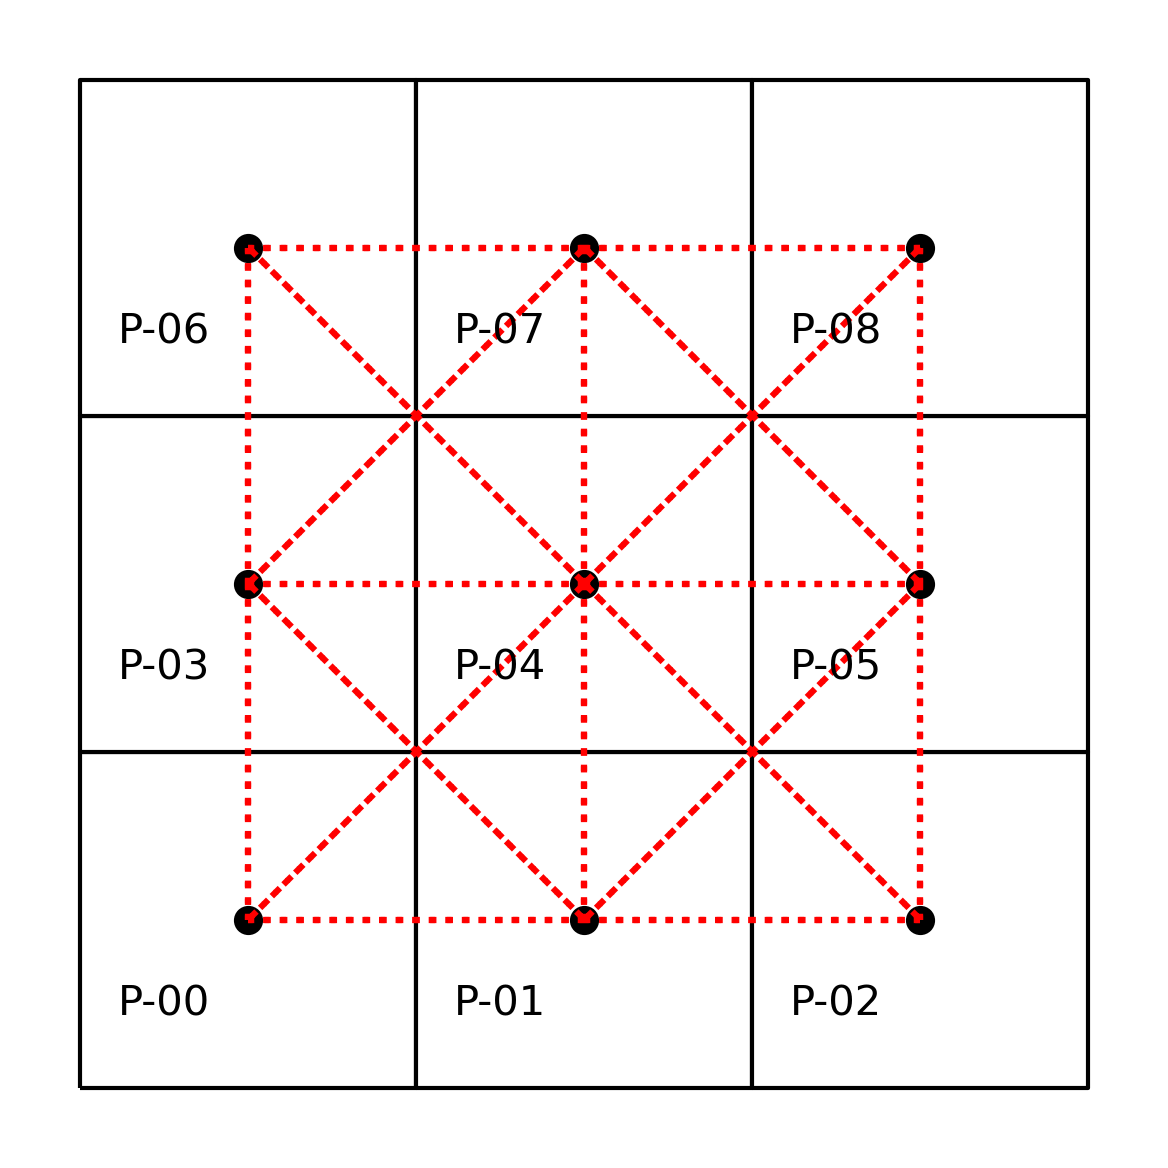
\includegraphics[width=0.4\textwidth]{assets/queens.png}
	\caption{Queens Model}
\end{figure}

Which has the following matrix attach to ti:
\[
	\begin{bmatrix}
		0 & 1 & 0 & 1 & 1 & 0 & 0 & 0 & 0 \\
		1 & 0 & 1 & 1 & 1 & 1 & 0 & 0 & 0 \\
		0 & 1 & 0 & 0 & 1 & 1 & 0 & 0 & 0 \\
		1 & 1 & 0 & 0 & 1 & 0 & 1 & 1 & 0 \\
		1 & 1 & 1 & 1 & 0 & 1 & 1 & 1 & 1 \\
		0 & 1 & 1 & 0 & 1 & 0 & 0 & 1 & 1 \\
		0 & 0 & 0 & 1 & 1 & 0 & 0 & 1 & 0 \\
		0 & 0 & 0 & 1 & 1 & 1 & 1 & 0 & 1 \\
		0 & 0 & 0 & 0 & 1 & 1 & 0 & 1 & 0 \\
	\end{bmatrix}
\]


There are also much more compress modell like the KNN model which followis the proces decreasing weights
as you become further way by K units away. You can see it in the folowing graph.

\begin{figure}[H]
	\centering
	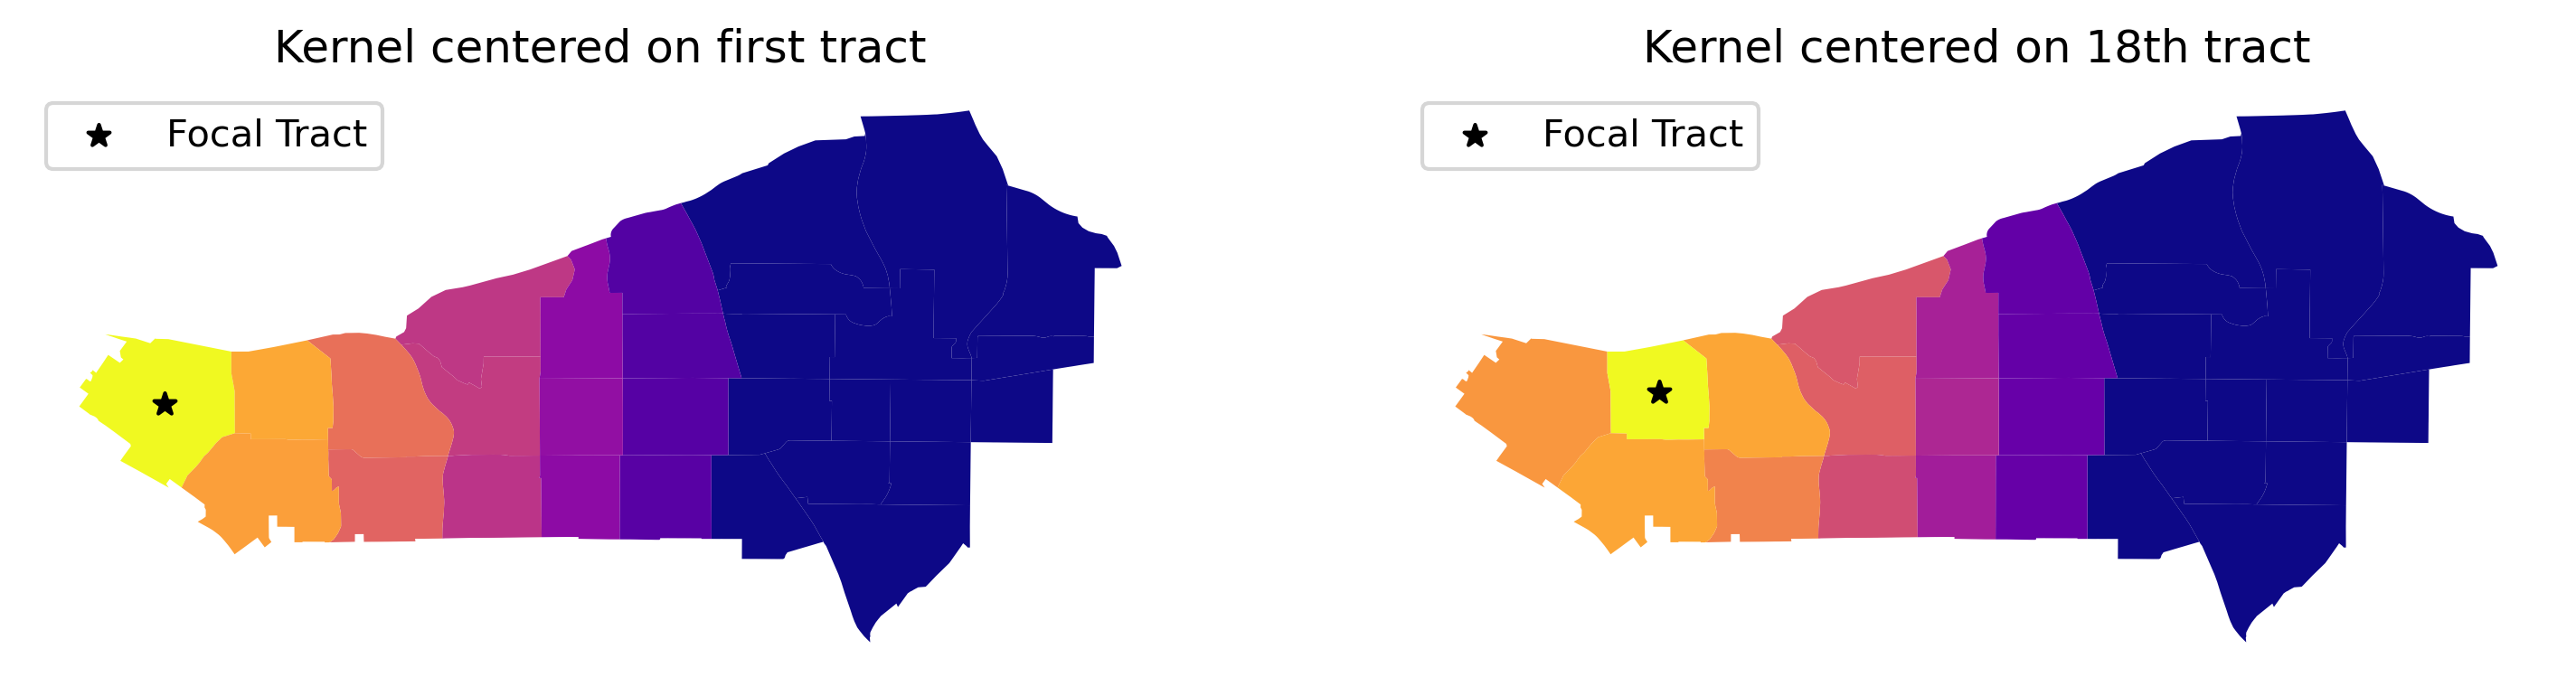
\includegraphics[width=0.64\textwidth]{assets/kmodel.png}
	\caption{KNN Model}
\end{figure}

It is clear to see that there numeruse ways to represent this $W$ matrix and no clear methode to deside which is apropiete
given that in practice $W$ is actualy an unknow given that when do not know the data generating proces.

\section{Research Plan and Methodology}

Starting for a simple regression of ordinary least squares (OLS) can be defined as follows:
\begin{equation}
	y_i = \alpha + \sum^p_{i=1} x_i \beta_i + \epsilon
	\label{eq:OLS}
\end{equation}
where $y$ is our expicatory variable and $x$ is the independent variables. If we wanted to study the corrolation that a location $i$ has on its neighbors, the classic approach would be
to define a relationship matrix $W$ which details how each location relates to all other locations. This classic Spatial regressions are an extension of the normal regresion with with
the addition of a spatialy term, which can be defined as follows:
\begin{equation}
	y = X \beta + \rho W X + \epsilon
	\label{eq:SDM}
\end{equation}

expanding the matrixes we get the following:
\begin{equation}
	y_{it} = \alpha + \sum^p_{i=1} x_{it} \beta_i + \rho \sum^N_{j=1} w_{ij} x_{jt} +\epsilon
	\label{eq:SDM_exp}
\end{equation}

This spatial can be addapted spatialy control for either your dependent term
\begin{equation}
	y = \alpha + X \beta + \rho W Y + \epsilon
	\label{eq:SAR}
\end{equation}

Or even the error term

\begin{equation}
	\begin{split}
		y & =\alpha + X \beta + u  \\
		u & =\gamma W u + \epsilon
	\end{split}
	\label{eq:SEM}
\end{equation}

Continuing from the SDM we can express the model a non linear equation as follows:
\begin{equation}
	y = \alpha + \sum^p_{i=1} x_{it} \beta_i + f(C_i) + \epsilon
	\label{eq:tensor}
\end{equation}
where $C$ is the centroid of the observations and $f(C)$ is a function given the centroid of the individuals.



The overall hypothesis is whether the semiparametric methode preforms better
on average given that we do not have reason to believe what is $W$. We expect to find what are to mesure the effects of picking a wrong $W$
and wheather we can miticate them with using a spetial smoother.

\section{Prototype Design and Implementation}

The Strategy for this resarch is to simulate data in the folowing format:
\begin{equation}
	y \sim \alpha + \sum^p_{i=1} x_{it} \beta_i + \rho \sum^N_{j=1} w_{ij} x_{jt} + \epsilon
\end{equation}

Where $\epsilon \sim N(0,\sigma^2$ and $W$ is defined in multiple ways this could be show in the following examples:

\section{Success and Impact}

The SDM generaly carries the problem that is very influenced on how $W$ is defined and there is now systematic
methedology to pick an apropiet $W$. This task is mostly delegated to domain experties. Given that the semiparametric
model proposed does not depend on $W$ this research intends to look if this model has a better preformance than the SDM model.
Preformance of this model is primarly defined as:
\begin{equation}
	\frac{\sum_{n=1}^N(y_n-\hat{y}_{nSDM})^2}{N}; \quad \frac{(y-\hat{y}_{GAM})^2}{N}
	\label{eq:pref}
\end{equation}
where $N$ is the number of simulations, $y$ is the predetermine outcome variable that we picked before the simulations are run.
In addition we would also use look at the performance of $\beta$ which can be shown in the simal maner:
\begin{equation}
	\frac{(\beta-\hat{\beta}_{SDM})^2}{N}; \quad \frac{(\beta-\hat{\beta}_{GAM})^2}{N}
	\label{eq:pref2}
\end{equation}


%Add all relevant references as a bibliography.

\bibliographystyle{plain}
\bibliography{reference}


\end{document}

